\documentclass{article}

\usepackage[utf8]{inputenc}
\usepackage{float}
\usepackage{graphicx}
\usepackage{subfig}

\begin{document}


\title{Lab 3: Rasterization}

\author{Karl Johan Andreasson \and Erik Fahlén}

\maketitle

\begin{figure}
    \centering
    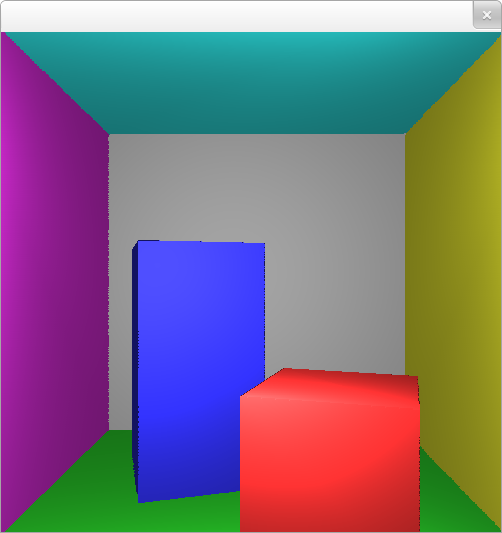
\includegraphics[width=10cm]{title.png}
    \caption{The scene rendered.}
    \label{fig:main}
\end{figure}

\section{Introduction}
As made evident in the laboration 2 one has to be very clever about the
implementation when using raytracers to make it render in real time.

To combat these massive computation times required by the raytracer a common
implementation method in computer graphics are to use rasterization.
Rasterization will provide a much faster rendering time for each frame making
the scene being rendered in real time. The real time aspect of rasterization is
making it an ideal approach for applications such as computer games. It is in
fact the most used method to draw frames in computer games.

There are disadvantages of using a rasterization, such as shadowing is much
harder to implement using rasterization than using ray tracing.

\section{Implementation method}

This laboration was implemented with both group members present and following
the instructions to implement the rasterization.

Since many of the concepts were familiar to us from completing laboration one
and two the initial parts of the laboration was completed rather quickly. The
depth buffer provided some difficulties but these were figured out without too
much of a delay.

When the calculation of the index of the left most and right most pixels in a
row on the screen was calculated for a triangle there were some issues were 
these indices were out of bounds leading to us trying to read bad memory
positions. Once we implemented checks to disregard the parts of the triangles 
that were not on the screen these issues were fixed.
\section{Discussion}
\section{Result}
\begin{figure}[H]
    \centering
    \begin{minipage}{.5\textwidth}
        \centering
        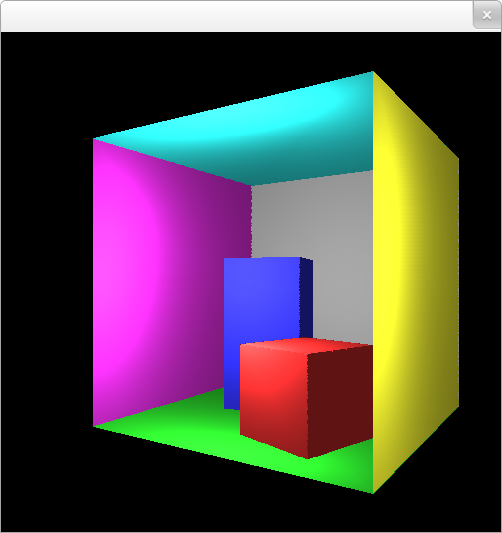
\includegraphics[width=4cm]{ani0.png}
    \end{minipage}%
    \begin{minipage}{.5\textwidth}
        \centering
        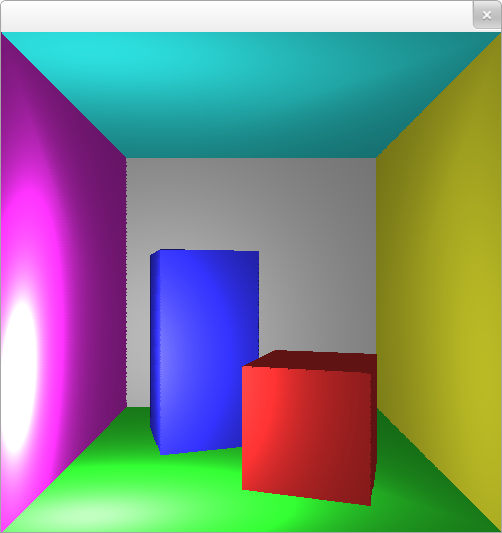
\includegraphics[width=4cm]{light0.png}
    \end{minipage}
\end{figure}

\begin{figure}[H]
    \centering
    \begin{minipage}{.5\textwidth}
        \centering
        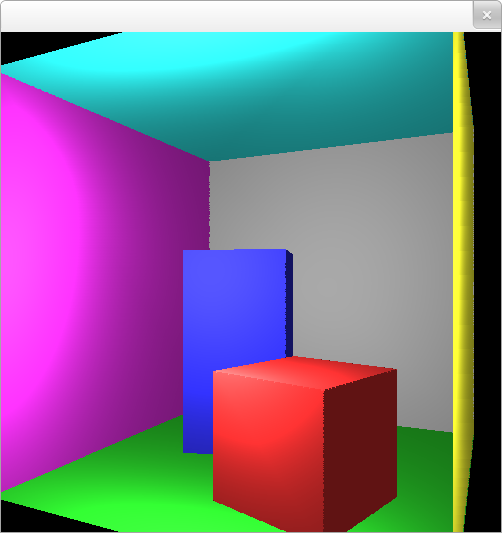
\includegraphics[width=4cm]{ani1.png}
    \end{minipage}%
    \begin{minipage}{.5\textwidth}
        \centering
        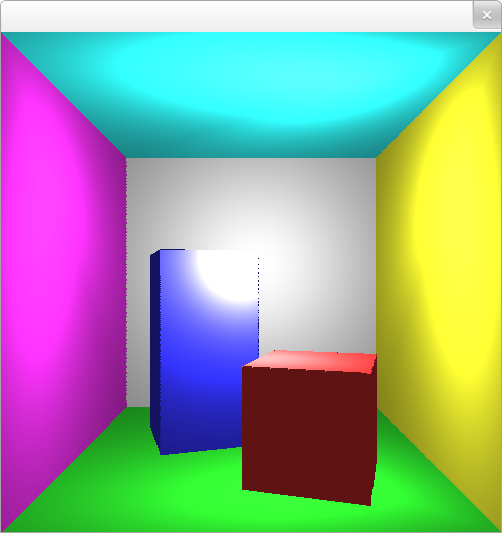
\includegraphics[width=4cm]{light1.png}
    \end{minipage}
\end{figure}

\begin{figure}[H]
    \centering
    \begin{minipage}{.5\textwidth}
        \centering
        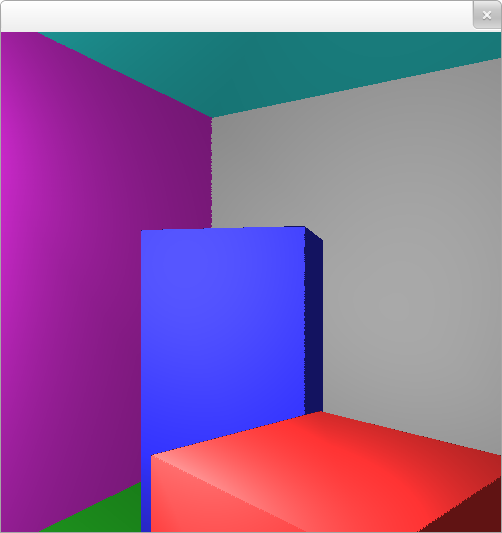
\includegraphics[width=4cm]{ani2.png}
        \captionof{figure}{\\Moving the camera around.}
        \label{fig:camera}
    \end{minipage}%
    \begin{minipage}{.5\textwidth}
        \centering
        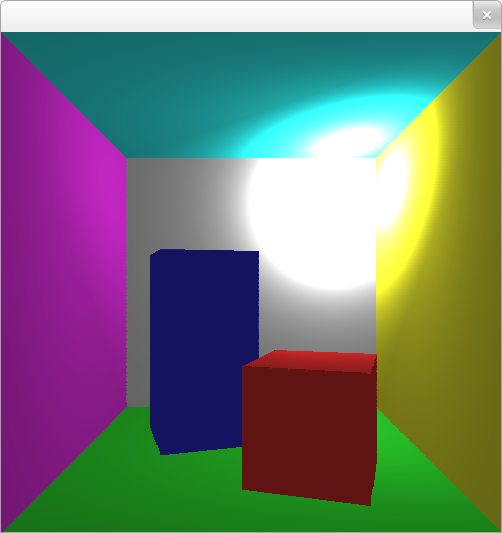
\includegraphics[width=4cm]{light2.png}
        \captionof{figure}{\\Moving the light source around.}
        \label{fig:light}
    \end{minipage}
\end{figure}

\end{document}
